\chapter[Referencial Teórico]{Referencial Teórico}

\section{Engenharia de Requisitos}

O conjunto de tarefas e técnicas utilizadas para promover o entendimento dos requisitos é denominado Engenharia de Requisitos. No desenvolvimento de software, pode ser vista como uma fase importante de Engenharia de Software que se inicia na atividade de comunicação e continua até a entrega do produto, sendo adaptada de acordo com as necessidades do processo de desenvolvimento, do produto e dos \textit{stakeholders} \cite{pressman2011engenharia}.

A Engenharia de requisitos abrange sete fases distintas: concepção, levantamento, elaboração, negociação, especificação, verificação e validação \cite{pressman2011engenharia}. De acordo com \cite{kotonya1998requirements} durante a execução das atividades das fases da Engenharia de Requisitos alguns problemas são relatados como: (i) Os requisitos não refletem as reais necessidades do cliente de acordo com o sistema a ser desenvolvido; (ii) São inconsistentes e/ou incompletos; (iii) É complexa a realização de alguma mudança no requisito, logo após terem sido acordado pelas partes; (iv) comumente é interpretado de maneira errada entre a equipe de desenvolvimento de software e o cliente.  

A maioria dos modelos dentro da Engenharia de Requisitos, não possuíam um tratamento adequado para tratar os atributos de qualidade, logo o tratamento desses atributos tem sido um foco chave de trabalhos na área da Engenharia de Requisitos Orientada a Meta \cite{chung2012non}. Entretanto neste trabalho é abordado o NFR \textit{framework} que trata os requisitos não funcionais em um nível mais alto de abstração, tanto para o problema quanto para a solução. 

\subsection{Engenharia de Requisitos Orientada a Meta}

Os requisitos de software muitas vezes são elicitados, modelados e analisados como metas ao qual os \textit{stakeholders} querem alcançar \cite{van2001goal}. Tipicamente as metas são elicitadas e conceituadas  em termos de alguma forma de modelo. Os modelos de metas têm sido utilizados como um meio eficaz para capturar as interações e os compromissos entre os requisitos \cite{letier2002deriving}. Além disso as metas podem contemplar diferentes tipos de interesses: interesses funcionais associados ao serviço que deverá ser prestado e interesses não funcionais associados a qualidade do serviço (precisão, desempenho, segurança) \cite{van2001goal}.
 
Para auxiliar no entendimento das metas podem ser realizados as seguintes perguntas "por que?", "como?", "de que outra forma?"\cite{van2001goal}. Onde o "por que?" auxilia na compreensão de objetivos superiores e logo se um requisito não é considerado, se não possuir uma contribuição para um objetivo superior; O "Como?" ajuda a entender as metas em níveis inferiores\cite{yu1998goal}; E "de que outra forma?" ajuda no processo de identificação de possíveis alternativas para o atendimento de metas superiores \cite{van2001goal}.  

\subsection{Requisitos Não-Funcionais}

Na literatura pode ser encontrada uma infinidade de definições para os NFRs, e vem sendo referenciados em termos que terminam com as palavras "-ilidades" ou "-idades", porém existem outros termos que referenciam requisitos não funcionais como por exemplo, desempenho, coerência, segurança, etc \cite{chung2012non}. Na área de arquitetura de software um termo frequentemente encontrado é atributos de qualidade \cite{barbacci1995quality}.

Sabendo disso os impactos diretos no tempo de execução, design do sistema e na experiência do usuário são diretamente ligados aos atributos de qualidade, o conjunto de atributos de qualidade representam as áreas de interesse que possuem grande impacto em seus níveis e camadas. Alguns atributos possuem impacto geral ao design do sistema (Exemplo: Suportabilidade) e outros atuam em problemas mais específicos (Exemplo: Usabilidade), é somente então quando a aplicação de software a ser desenvolvida atende uma combinação desejada desses atributos que o sucesso do design e a qualidade geral do aplicativo de software é atingida\cite{microsoft2009}.


\section{NFR Framework}

O NFR Framework é um modelo intencional que ajuda desenvolvedores e engenheiros de requisitos a lidarem com requisitos não-funcionais, através de um grafo chamado de Softgoal Interdependency Graphs - SIGs, onde os requisitos podem ser analisados pois o mesmo, permite uma visão vertical desde a estratégia de alto nível até os detalhes operacionais;  possuindo operadores lógicos AND (E) e OR (OU) que promovem uma melhor tomada de decisão; onde  os requisitos não funcionais são escritos através de uma notação formal que permite provar a sua correção e completude. O framework também possui uma estrutura que pode ser orientada por processo, dando suporte às atividades do processo de engenharia de requisitos e pode ser utilizado como complemento nas abordagens tradicionais de desenvolvimento de software \cite{chung2012non}.

O NFR Framework utiliza o conceito de metas flexíveis que é uma condição ou estado no mundo real que deseja ser alcançado, podendo assumir natureza subjetiva, pois o RNF pode variar de acordo com o julgamento de cada pessoa; e natureza relativa, pois o RNF pode depender de algum tipo de relação com outro RNF.  A notação no SIGs para a meta flexível é uma nuvem como mostra a figura \ref{fig01}, que também pode representar uma operacionalização e também uma reivindicação.

\begin{figure}[h]
	\centering
	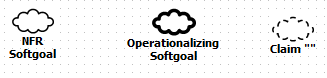
\includegraphics[keepaspectratio=true,scale=0.9]{figuras/tiposDeSoftgoals.png}
	\caption{Representação gráfica dos tipos de \textit{metas flexíveis}.}
	\label{fig01}
\end{figure} 

Para facilitar o entendimento das decisões tomadas a meta flexível possui labels que determinam o grau em que determinado RNF é satisfeito de acordo com um conjunto de decisões do projeto, essas labels são: satisfeita, fracamente satisfeita,  negada, fracamente negada, crítica e indecisa \cite{chung2012non}.Outra notação importante é o grau de prioridade de uma meta flexível, representada por “\textbf{!}” ou “\textbf{!!}” para um grau de prioridade maior.

\begin{figure}[h]
	\centering
	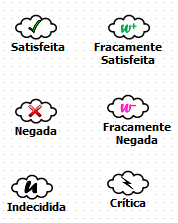
\includegraphics[keepaspectratio=true,scale=0.9]{figuras/labelsSoftgoals.png}
	\caption{Representação gráfica das labels das \textit{metas flexíveis}.}
	\label{fig02}
\end{figure} 

As relações que as metas flexíveis possuem uma com as outras é estabelecida através de interdependências, são as interdependências que realizam o registro do refinamento das metas flexíveis em metas flexíveis mais específicas (filhos) e de certa forma, contribui para satisfazer a meta flexível mais genérica (pai), os tipos de contribuição são apresentados na tabela abaixo \cite{chung2012non}.

\begin{table}[h]
	\centering
	\caption{Tipos de contribuições.}
	\label{tiposDeContribuições}
	\begin{tabular}{|l|l|}
		\hline
		\textbf{Símbolo} & \textbf{Descrição} \\ \hline
		\multirow{2}{*}{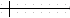
\includegraphics[scale=0.9]{figuras/And.png}} & \multirow{2}{*}{AND: Se todos os filhos são satisfeitos o pai também será satisfeito.} \\
		&  \\ \hline
		\multirow{2}{*}{\includegraphics[scale=0.9]{figuras/OR.png}} & \multirow{2}{*}{OR: Se qualquer filho é satisfeito o pai também será satisfeito.} \\
		&  \\ \hline
		\multirow{2}{*}{
\includegraphics[scale=0.9]{figuras/Make.png}} & \multirow{2}{*}{\begin{tabular}[c]{@{}l@{}}MAKE: Pode ser tratado de forma semelhante ao AND, pois se \\ o filho for satisfeito o pai pode ser satisfeito.\end{tabular}} \\
		&  \\ \hline
		\multirow{2}{*}{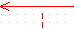
\includegraphics[scale=0.9]{figuras/Break.png}} & \multirow{2}{*}{\begin{tabular}[c]{@{}l@{}}BREAK: Fornece apoio negativo, pois se o filho é satisfeito o \\ pai pode ser negado.\end{tabular}} \\
		&  \\ \hline
		\multirow{2}{*}{
\includegraphics[scale=0.9]{figuras/Help.png}} & \multirow{2}{*}{HELP: Se todos os filhos são satisfeitos o pai também será satisfeito.} \\
		&  \\ \hline
		\multirow{2}{*}{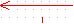
\includegraphics[scale=0.9]{figuras/Hurt.png}} & \multirow{2}{*}{HURT: Se todos os filhos são satisfeitos o pai será fracamente negado.} \\
		&  \\ \hline
		\multirow{2}{*}{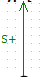
\includegraphics[scale=0.9]{figuras/SomeMais.png}} & \multirow{2}{*}{SOME+: Representa a existência de alguma contribuição positiva.} \\
		&  \\ \hline
		\multirow{2}{*}{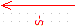
\includegraphics[scale=0.9]{figuras/SomeMenos.png}} & \multirow{2}{*}{SOME-: Representa a existência de alguma contribuição negativa.} \\
		&  \\ \hline
	\end{tabular}
\end{table}

A figura \ref{exemploNFR} apresenta uma decomposição de uma meta flexível em outras metas de mesma natureza, consideramos então neste exemplo o RNF: “manter as contas com boa segurança” onde a meta flexível  “segurança de contas” é refinada em outras como: “Integridade de contas”, “Confidencialidade de contas” e “Disponibilidade de contas” \cite{chung2012non}.

\begin{figure}[h]
	\centering
	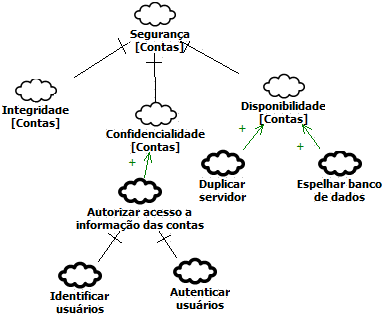
\includegraphics[keepaspectratio=true,scale=1.0]{figuras/exemploNFR.png}
	\caption{Operacionalização de segurança de contas adapatado de \cite{chung2012non}, \cite{affleck2012supporting}.}
	\label{exemploNFR}
\end{figure} 

Confidencialidade de contas é operacionalizada em “Autorizar acesso a informação das contas” que possui uma contribuição do tipo HELP com seu pai, para que essa operacionalização seja satisfeita seus filhos devem ser satisfeitos devido a relação do tipo AND ao ser operacionalizada em “Identificar usuários” e “Autenticar usuários”.

Para Disponibilidade de contas a mesma é operacionalizada em “Duplicar servidor” e “Espelhar banco de dados” essas operacionalizações possuem contribuições do tipo HELP e mesmo pai, e para a meta flexível ser satisfeita, ambas as operacionalizações devem ser satisfeitas \cite{affleck2012supporting}. 



\subsection{i*}



\subsection{FURPS}


\section{Arquitetura de Software}

\subsection{MVC - Model-View-Controller}

\chapter{Metodologia}

\subsection{Classificação da Pesquisa}